% Drawing 148/02-3 -- folder 148, batch 02, archive page 22 (PDF page 23).
% Transcription: à droite des deux groupes, un grand réseau triangulaire dessiné dans un parallélogramme ; des traits repassés en gras (deux obliques, deux horizontaux) y délimitent un parallélogramme fondamental, avec deux flèches de translation issues d'un même sommet marqué ; une partie du réseau est hachurée.
% Kind: triangular lattice with a heavy fundamental parallelogram and two translation arrows. Method 2 (schematic redraw from the facsimile). Status: partial.
% Notes: Ink, much overdrawn. A parallelogram filled with a triangular lattice (three families of lines), drawn here as a regular lattice of nine cells by seven rows fitted to the outline. Over it, as on the page: two heavy oblique strokes parallel to the left side, the first ending in an arrowhead at the top; two heavy horizontal strokes, the lower one ending in an arrowhead on the right; a heavy dot where the first oblique stroke meets the lower horizontal one. Left out: the scribbled hatching over the cells left of the heavy dot. Still differs: the lattice on the page is irregular, and the heavy strokes are placed by eye on it, so that which lattice points the fundamental parallelogram joins cannot be read off the redraw; the count of cells (nine by seven) is approximate. Redrawn 2026-11-12 (issue 128): to check again.
% Coordinates: 1 unit = 1 mm = 1/100 of the crop width, y downwards as on the crop (bbox in page fractions: [0.44, 0.455, 0.8, 0.6]).
% Redrawn by Claude (claude-fable-5-2), issue #128, 2026-11-12; not checked by a human; not compiled (no TeX in the session).
% Rights: reproduces part of the work -- behind RENDER_TRANSCRIPTS, never published by itself.
\documentclass[tikz,border=3pt]{standalone}
\usepackage{amsmath,amssymb}
\usetikzlibrary{patterns,arrows.meta}
\tikzset{pencil/.style={black!45}, struck/.style={black!35}, mpt/.style={circle,draw,inner sep=1.3pt}, pt/.style={circle,fill,inner sep=0.9pt}, opt/.style={circle,draw,fill=white,inner sep=1.1pt}, Rd/.style={red!75!black}, Gn/.style={green!45!black}, Br/.style={brown!70!black}}
\begin{document}
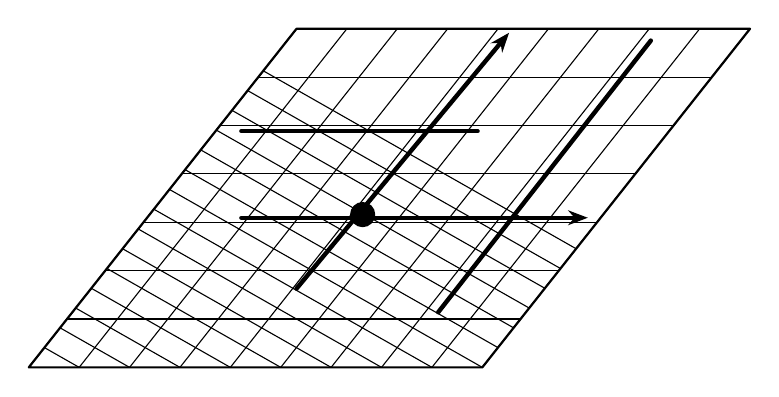
\begin{tikzpicture}[x=1mm,y=-1mm,line cap=round,line join=round,font=\small]
\begin{scope}
\clip (3,52) -- (60.6,52) -- (94.6,9) -- (37,9) -- cycle;
\foreach \j in {0,...,7} {
\draw[thin] (3+4.857*\j,52-6.143*\j) -- (60.6+4.857*\j,52-6.143*\j);
}
\foreach \i in {0,...,9} {
\draw[thin] (3+6.4*\i,52) -- (37+6.4*\i,9);
}
\foreach \k in {1,...,15} {
\draw[thin] (3+6.4*\k,52) -- (3+6.4*\k-10.801*7,52-6.143*7);
}
\end{scope}
\draw[thick] (3,52) -- (60.6,52) -- (94.6,9) -- (37,9) -- cycle;
\draw[line width=1.6pt,-{Stealth[length=2.5mm]}] (37,42) -- (64,9.5);
\draw[line width=1.6pt] (55,45) -- (82,10.5);
\draw[line width=1.6pt] (30,22) -- (60,22);
\draw[line width=1.6pt,-{Stealth[length=2.5mm]}] (30,33) -- (74,33);
\fill (45.4,32.6) circle [radius=1.6];
\end{tikzpicture}
\end{document}
